В этом примере три команды ($N = 3$) и $8$ секторов ($L = 8$), а Аман может держать в руках
два сувенира ($K = 2$). Команды находятся в секторах с номерами $1$, $2$ и $5$.

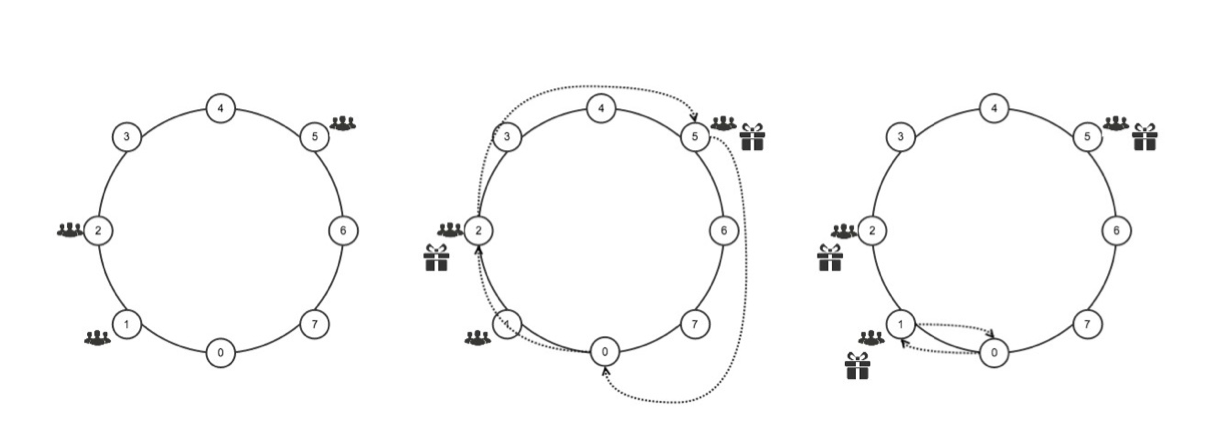
\includegraphics[scale=0.8]{boxes1.png}

Одно из оптимальных решений показано на рисунке выше. За первый проход Аман берет два
сувенира, передает один сувенир команде в секторе $2$, второй~--- команде в секторе $5$, а затем
возвращается в сектор $0$. Этот проход занимает у него $8$ секунд. За второй проход Аман
доставляет оставшийся сувенир команде в секторе $1$ и возвращается в сектор $0$. На это он
тратит еще $2$ секунды. Суммарное время доставки $10$ секунд
